\documentclass[a0paper, 25pt, portrait, margin=10mm, innermargin=15mm, blockverticalspace=15mm, colspace=15mm]{tikzposter}

% --- Theme and Color ---
\usetheme{Envelope} % More dynamic theme
% \usecolortheme{Blue} % Removed - Not a standard command

% --- Packages from Paper & Poster ---
\usepackage{amsmath,amssymb,amsthm}
\usepackage{graphicx}
\usepackage{booktabs}
\usepackage{xcolor} % tikzposter uses xcolor
\usepackage[hidelinks]{hyperref}
\usepackage{url}
\usepackage{caption} % Needed for \captionof
\usepackage{pifont} % Needed for \ding symbols

% --- Custom Commands from Paper ---
\newcommand{\avg}{\text{avg}}
\newcommand{\km}{\kappa_\phi}
\newcommand{\res}{\text{res}}
\newcommand{\E}{\mathbb{E}\,}
\newcommand{\R}{\mathbb{R}}
\newcommand{\he}{\mathrm{he}}
\newcommand{\He}{\mathrm{He}}

% --- Theorem Environments from Paper ---
\newtheorem{theorem}{Theorem}
\newtheorem{lemma}{Lemma}
\newtheorem{remark}{Remark}
\newtheorem{corollary}{Corollary}
\newtheorem{proposition}{Proposition}
\theoremstyle{definition}
\newtheorem{definition}{Definition}

% --- Poster Specific Settings ---
\graphicspath{ {./figures/} } % Set path for figures
\definecolor{TPhighlight}{rgb}{0.2,0.5,0.8} % Example: Define a custom highlight color (used below)

% --- Title, Author, Institute ---
% \title{ Emergence of Globally Attracting Fixed Points in\newline
% Deep Neural Networks With Nonlinear Activations} % More engaging 
\title{ \parbox{\linewidth}{ \centering Emergence of Globally Attracting Fixed Points in\\ Deep Neural Networks With Nonlinear Activations}}



\author{Amir Joudaki \quad Thomas Hofmann}
\institute{Department of Computer Science, ETH Zürich \\ \vspace{1mm} {\small AISTATS 2025 -- Zürich, Switzerland -- April 27, 2025}} % Added conference/date context
% \titlegraphic{\includegraphics[width=0.12\linewidth]{ETH_logo_white.png}} % Optional: Add ETH/AISTATS logo (replace placeholder_logo.png with your file, maybe needs white bg)

\begin{document}

\maketitle \vspace{-10mm} % Adjust spacing after title if needed

\begin{columns} % Start columns environment

% === COLUMN 1: Motivation & Problem Setup ===
\column{0.32}

\block{Why Study Representation Similarity in in depth?}{
    Deep nonlinear nets are powerful function approximators, but \emph{how} they transform inputs layer-by-layer remains mysterious. Understanding this is key to:
    \begin{itemize}
        \item Demystifying role of nonlinear activations.
        \item Make choice of activations more principled.
        \item Demystifying how depth and nonlinearity interact to shape input  similarity at initializtion
    \end{itemize}
    A crucial aspect is how the similarity between representations of different inputs evolves with depth as a function of the non-linearity function. Does it vanish? Saturate? Depend fundamentally on the activation function?
    \\[2mm]
    \textbf{Our Goal:} Analyze the global, layer-wise evolution of representation similarity at initialization.
}

\block{Problem Setup: The Kernel Sequence}{
    We study a standard MLP:
    $$ h^\ell(x) = \phi\left(\frac{1}{\sqrt{d}}W^\ell h^{\ell-1}(x)\right) $$
    where $\phi$ is the activation and $W^\ell$ are random weight matrices (zero mean, unit variance entries).

    The core quantity is the \textbf{Neural Kernel} (normalized inner product) at layer $\ell$:
    $$ \rho_\ell(x,y) = \langle h^\ell(x), h^\ell(y) \rangle_\avg $$
    We analyze the \textbf{kernel sequence} $\{\rho_\ell\}_{\ell \ge 0}$ as $\ell \to \infty$.
    We assume \textbf{forward stability}: $\E[\phi(X)^2]=1$ for $X \sim \mathcal{N}(0,1)$.
}

\block{The Key Idea: Mean-Field + Hermite}{
    \textbf{1. Mean-Field Limit ($d \to \infty$):} Randomness averages out! The kernel evolution becomes deterministic.
    \begin{proposition}[Deterministic Evolution]
        $\rho_{\ell+1} = \km(\rho_\ell)$
    \end{proposition}
    The dynamics are governed by the \textbf{Kernel Map} $\km$:
    \begin{definition}[Kernel Map $\km$] \label{def:kernel_map}
        For $(X, Y) \sim \mathcal{N}(0, \begin{pmatrix} 1 & \rho \\ \rho & 1 \end{pmatrix})$: $\km(\rho) := \E[\phi(X)\phi(Y)]$
    \end{definition}

    \textbf{2. Hermite Polynomials:} The natural basis for functions under Gaussian measures.
    $$ \phi(x) = \sum_{k=0}^\infty c_k \he_k(x) \quad (c_k = \E[\phi(X)\he_k(X)]) $$
    Mehler's Lemma ($\E[\he_m(X)\he_n(Y)] = \rho^n \delta_{mn}$) yields:
    \begin{corollary}[Explicit Kernel Map]
        $$ \boxed{\km(\rho) = \sum_{k=0}^\infty c_k^2 \rho^k} $$
        An elegant power series determined \emph{only} by the activation's Hermite coefficients ($c_k^2$)!
    \end{corollary}
}

% === COLUMN 2: Main Result & Implications ===
\column{0.36} % Slightly wider column for the main result and figures

\block{\bfseries The Surprising Result: Global Convergence}{
    \begin{theorem}[Global Attraction] \label{thm:global_attract}
    For \textbf{any non-linear} activation $\phi$ (with $\km(1)=1$) and any initial similarity $\rho_0 \in (-1, 1)$, the kernel sequence $\rho_\ell$ \textbf{converges globally} to a \textbf{single, unique attracting fixed point} $\rho^* \in [0, 1]$.
    \end{theorem}
    \vspace{-3mm} % Adjust spacing
    \centerline{\color{TPhighlight}\rule{0.8\linewidth}{1pt}} % Visual separator
    \vspace{1mm} % Adjust spacing
    This fixed point reveals an \textbf{inherent implicit bias} determined by the activation function:

    \textbf{Four Types of Convergence Behavior:}
    \begin{enumerate}
        \item[\Large \ding{108}] \textbf{Orthogonality Bias ($\rho^*=0$):} If $\km(0)=0$. Representations become orthogonal exponentially fast. (\textit{e.g., tanh, SeLU})
        \item[\Large \ding{109}] \textbf{Strong Similarity Bias ($\rho^*=1$):} If $\km(0)>0$ \& $\km'(1)\le 1$. Representations become highly aligned (exponentially if $\km'(1)<1$, polynomially if $\km'(1)=1$). (\textit{e.g., ReLU, sigmoid, exp})
        \item[\Large \ding{110}] \textbf{Weak Similarity Bias ($\rho^* \in (0,1)$):} If $\km(0)>0$ \& $\km'(1) > 1$. Representations converge to a non-trivial, intermediate similarity. (\textit{e.g., GELU, ELU})
    \end{enumerate}
     \centerline{\color{TPhighlight}\rule{0.8\linewidth}{1pt}} % Visual separator
    \vspace{1mm} % Adjust spacing
    \textbf{Implication:} Deep networks, even at initialization, are intrinsically biased towards making inputs either very distinct, very similar, or moderately similar, depending \emph{only} on $\phi$.
}

\block{Validation: Theory Meets Practice}{
    We plot the kernel map $\km(\rho)$ and the convergence trajectory $\rho_\ell$ vs. depth $\ell$.
    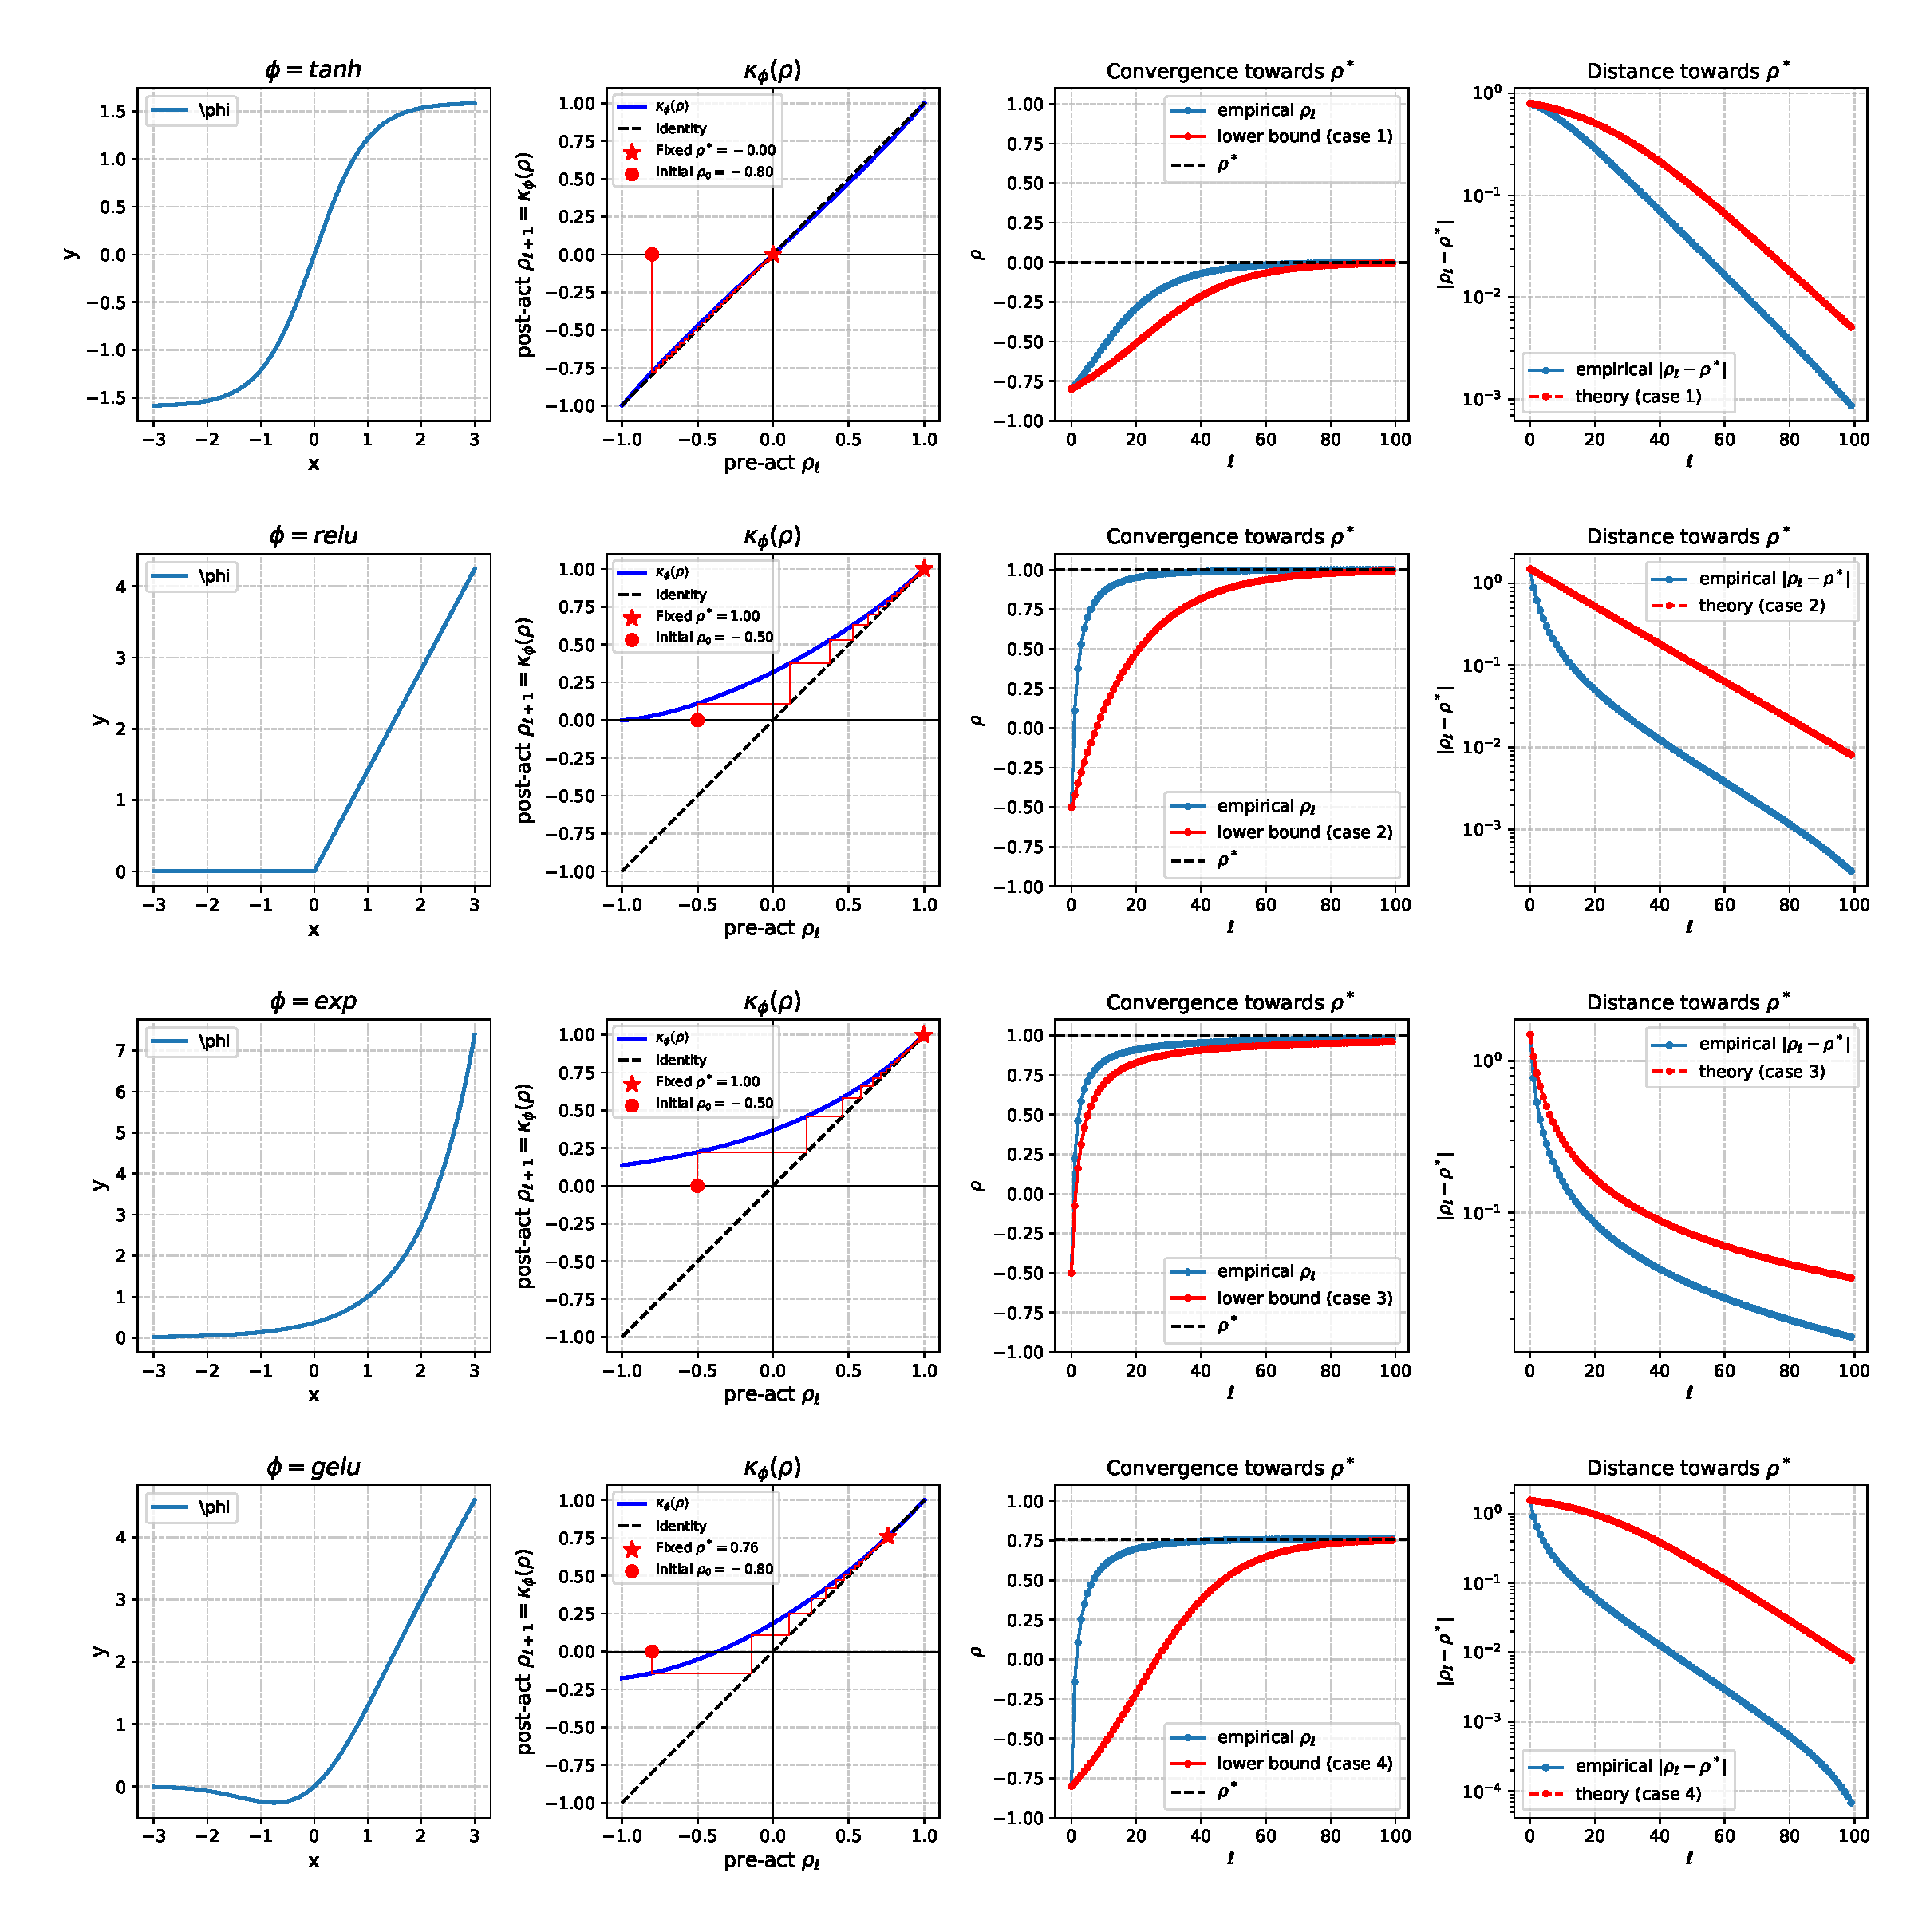
\includegraphics[width=0.98\linewidth]{kernel_convergence} % Needs kernel_convergence.pdf
    \vspace{2mm}
    % 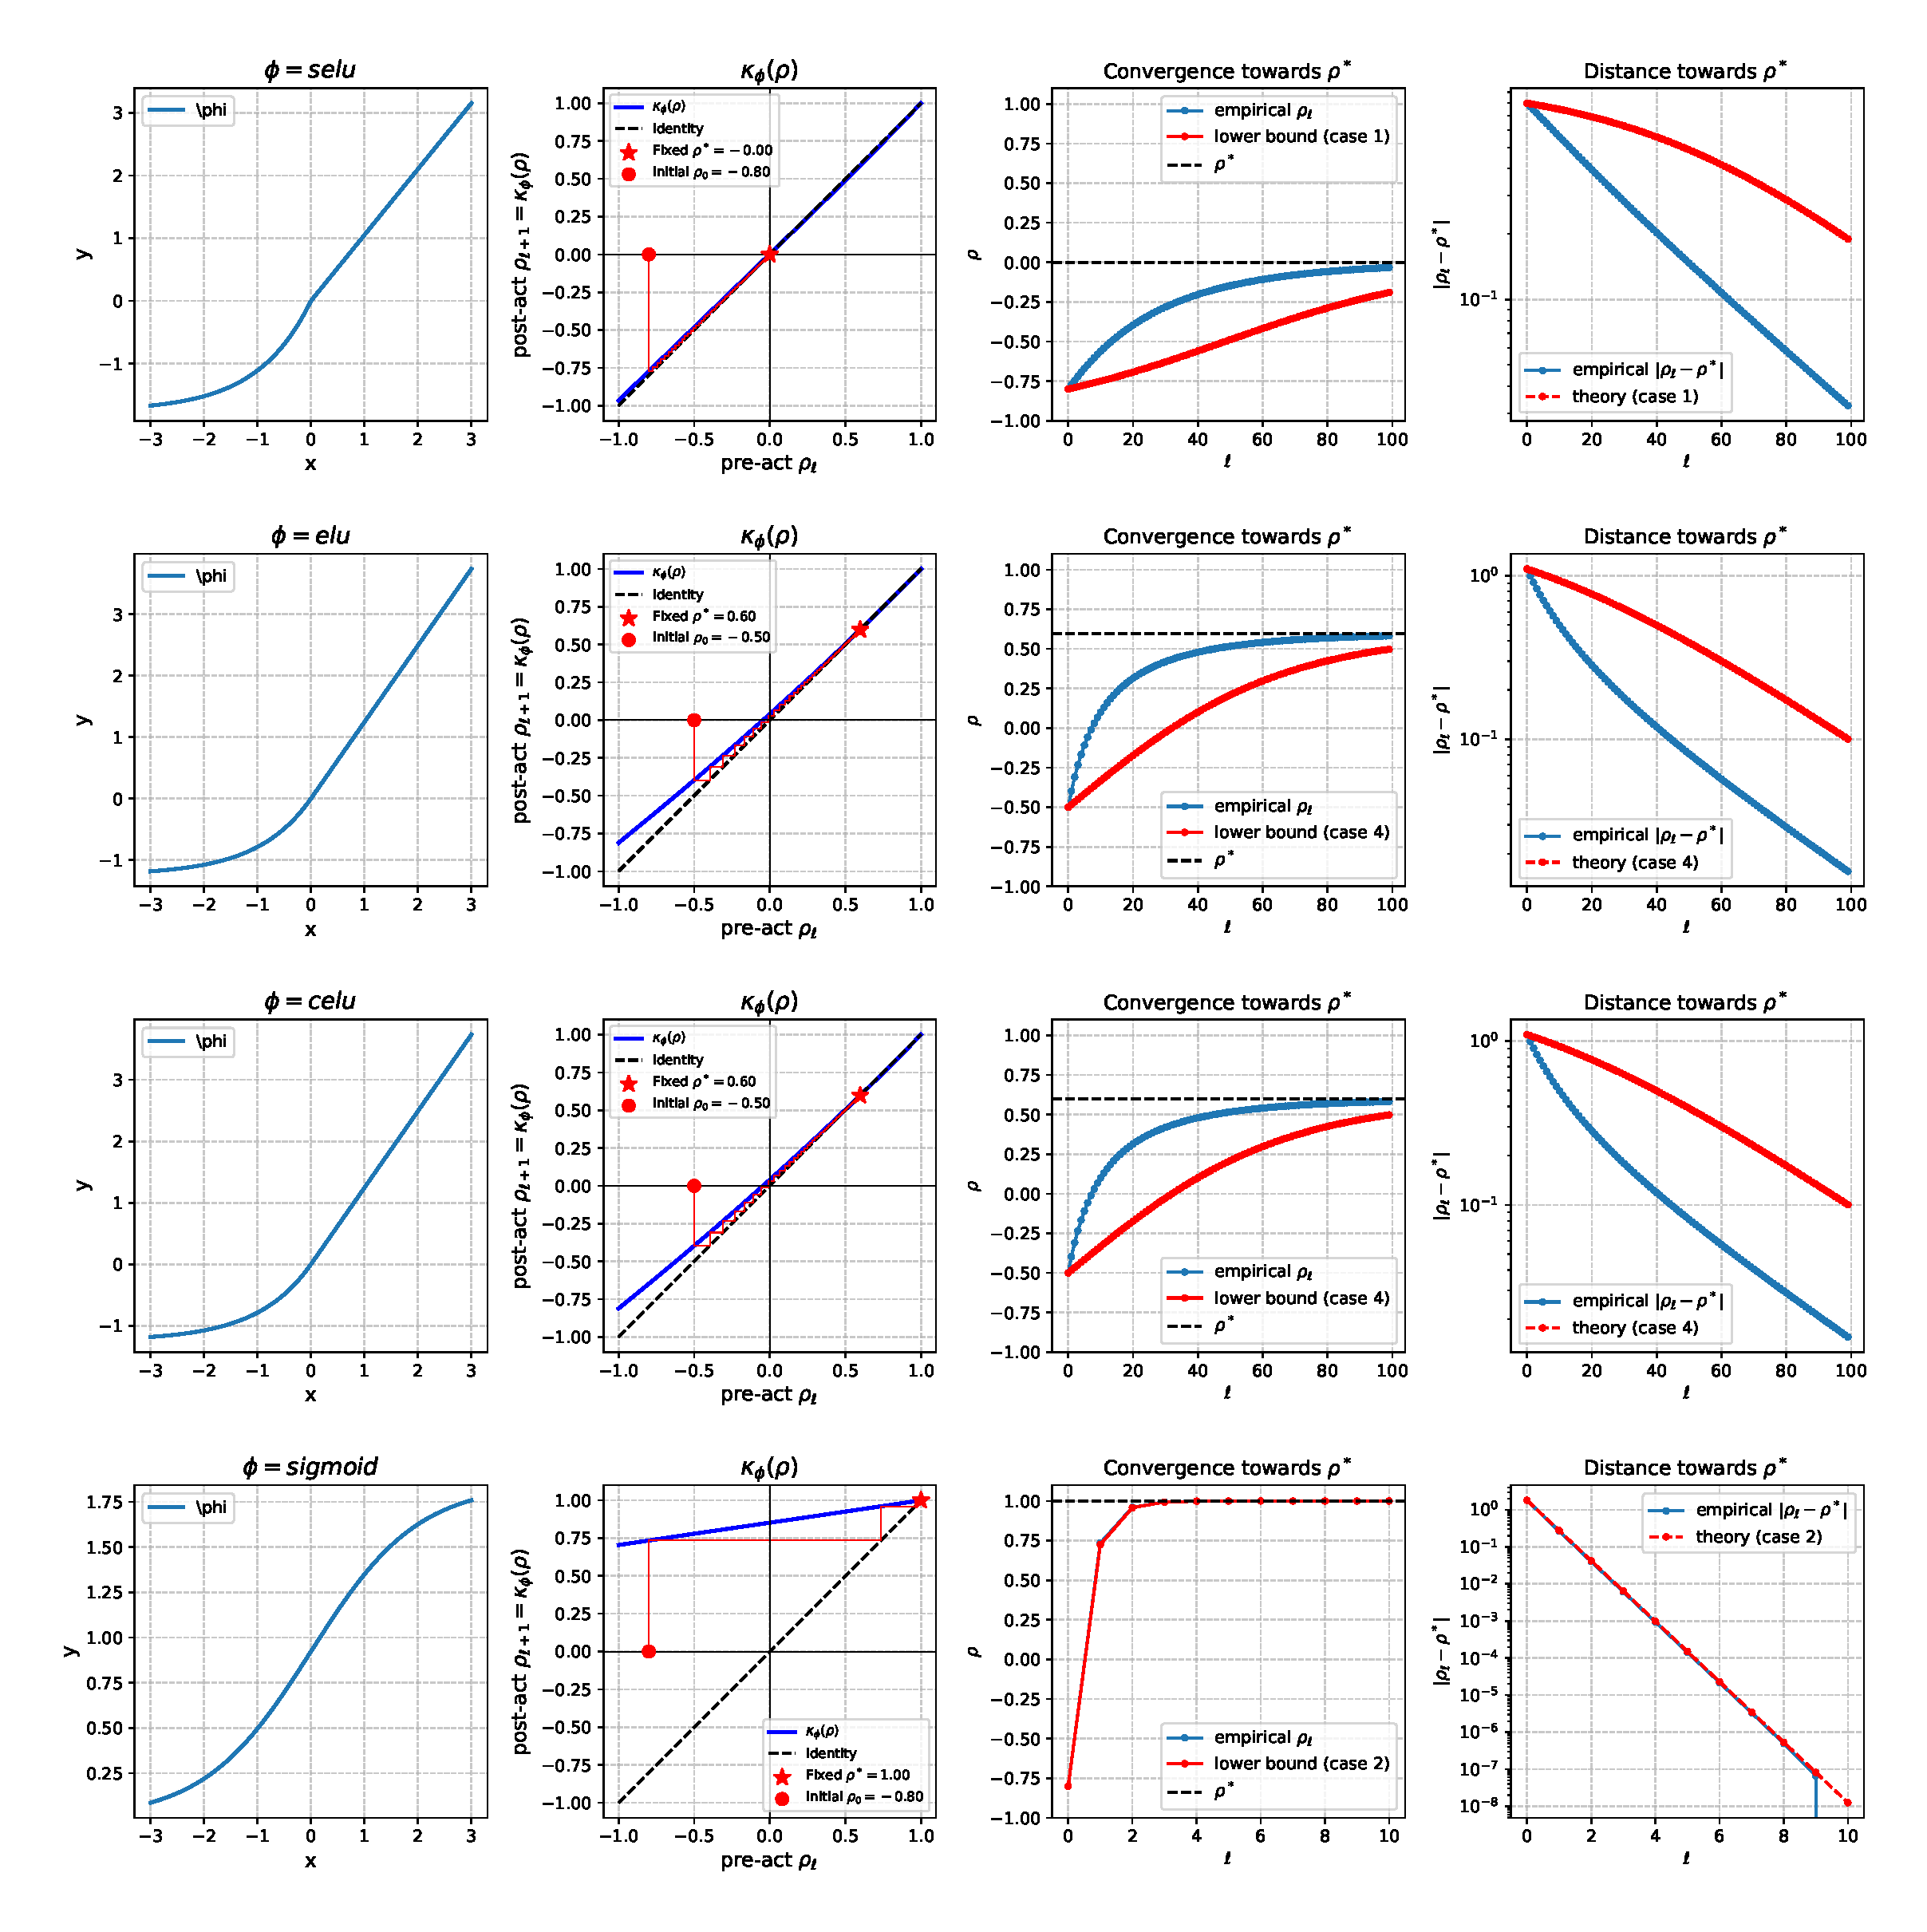
\includegraphics[width=0.98\linewidth]{kernel_convergence_2} % Needs kernel_convergence_2.pdf
    \textit{Observations:} Empirical convergence matches theoretical predictions (fixed points, exponential/polynomial decay). The Hermite analysis accurately captures the dynamics.
}

% === COLUMN 3: Extensions & Takeaways ===
\column{0.32}

\block{What About ResNets \& Normalization?}{
    Our framework extends easily:

    \textbf{Residual Connections (Strength $r$):}
    $\kappa_\res(\rho) = (1-r^2)\km(\rho) + r^2 \rho$.
    \begin{itemize}
        \item Same fixed points $\rho^*$.
        \item \textbf{Slows down} convergence. Residuals counteract the activation's bias.
    \end{itemize}

    \textbf{Normalization Layers:}
    \begin{itemize}
        \item RN or LN \emph{before} $\phi$: No change to $\km$ in mean-field.
        \item \textbf{LN \emph{after}} $\phi$: Transforms map to $\kappa_\psi(\rho) = \frac{\km(\rho) - \km(0)}{1 - \km(0)}$.
        \textit{Key Effect:} Centers the map ($\kappa_\psi(0)=0$), forcing an \textbf{orthogonality bias ($\rho^*=0$)} regardless of $\phi$'s original bias! Explains benefits seen in practice.
    \end{itemize}
}

\block{Activation Properties \& Biases}{
    \centering
    \resizebox{0.95\linewidth}{!}{% Make table fit
    \begin{tabular}{lccc}
    \toprule
    $\phi$ (normalized) & Attracting FP $\rho^*$ & Bias Type & Case \\
    \midrule
    \texttt{tanh} & 0.00 & Orthogonality & 1 \\
    \texttt{SeLU} & 0.00 & Orthogonality & 1 \\
    \texttt{ReLU} & 1.00 & Strong Similarity & 2 \\
    \texttt{sigmoid} & 1.00 & Strong Similarity & 2 \\
    \texttt{exp} & 1.00 & Strong Similarity & 3 \\
    \texttt{GELU} & 0.76 & Weak Similarity & 4 \\
    \texttt{ELU} & 0.60 & Weak Similarity & 4 \\
    \bottomrule
    \end{tabular}
    } % end resizebox
    \captionof{table}{Implicit bias induced by common activations (Thm \ref{thm:global_attract}).}
    \label{tab:activation_stats_poster}
}

\block{Key Insights \& Impact}{
    \begin{itemize}
        \item[\Large \checkmark] Deep networks exhibit \textbf{global convergence} of representation similarity at initialization.
        \item[\Large \checkmark] This convergence leads to a \textbf{unique fixed point} determined solely by the activation function.
        \item[\Large \checkmark] \textbf{Hermite polynomials} provide the mathematical key to unlock and predict these dynamics explicitly.
        \item[\Large \checkmark] Reveals fundamental \textbf{implicit biases} (orthogonality/similarity) baked into network architectures.
        \item[\Large \checkmark] Explains how \textbf{residuals slow down} convergence and \textbf{LayerNorm (post) forces orthogonality}.
        \item[\Large \checkmark] Offers a principled way to understand the interplay of depth, non-linearity, and architectural choices.
    \end{itemize}
}

\block{Contact \& Code}{
    \textbf{Amir Joudaki}: \texttt{amir.joudaki@inf.ethz.ch} \\
    \vspace{2mm}
    Code available at: \\
    \url{https://github.com/ajoudaki/kernel-global} \\
    % \qrcode[height=1.5cm]{https://github.com/ajoudaki/kernel-global} % Optional QR Code
}

\end{columns} % End columns environment

\end{document}